\documentclass{VUMIFInfKursinis}
\usepackage{algorithmicx}
\usepackage{algorithm}
\usepackage{algpseudocode}
\usepackage{amsfonts}
\usepackage{amsmath}
\usepackage{bm}
\usepackage{color}
\usepackage{graphicx}
% \usepackage{hyperref}  % Nuorodų aktyvavimas
\usepackage{url}


% Titulinio aprašas
\university{Vilniaus universitetas}
\faculty{Matematikos ir informatikos fakultetas}
\institute{Informatikos institutas}  % Užkomentavus šią eilutę - institutas neįtraukiamas į titulinį
\department{Informatikos katedra}
\papertype{Operacinių sistemų pirmoji užduotis}
\title{Virtualios ir realios mašinos projektas}
%\titleineng{Modeling of Risk Management Process}
\status{3 kurso 1 grupės studentas}
\author{Dominykas Marma}
% \secondauthor{Vardonis Pavardonis}   % Pridėti antrą autorių
\supervisor{Mantas Grubliauskis}
\date{Vilnius \\ \the\year}

% Nustatymai
% \setmainfont{Palemonas}   % Pakeisti teksto šriftą į Palemonas (turi būti įdiegtas sistemoje)
\bibliography{bibliografija} 

\begin{document}
\maketitle

\tableofcontents

\section{Užduoties aparašymas}

Virtualios mašinos procesoriaus komandos operuoja su duomenimis, esančiais registruose ir ar atmintyje. Yra komandos duomenų persiuntimui iš atminties į registrus ir atvirkščiai, aritmetinės (sudėties, atimties, daugybos, dalybos, palyginimo), sąlyginio ir besąlyginio valdymo perdavimo, įvedimo, išvedimo, darbo su failais (atidarymo, skaitymo, rašymo, uždarymo, sunaikinimo) ir programos pabaigos komandos. Registrai yra tokie: komandų skaitiklis, bent du bendrosios paskirties registrai, požymių registras (požymius formuoja aritmetinės, o į juos reaguoja sąlyginio valdymo perdavimo komandos). Atminties dydis yra 16 blokų po 16 žodžių (žodžio ilgį pasirinkite patys).

Realios mašinos procesorius gali dirbti dviem režimais: vartotojo ir supervizoriaus. Virtualios mašinos atmintis atvaizduojama į vartotojo atmintį naudojant puslapių transliaciją. Yra taimeris, kas tam tikrą laiko intervalą generuojantis pertraukimus. Įvedimui naudojama klaviatūra, išvedimui - ekranas. Yra išorinės atminties įrenginys - kietasis diskas.

Vartotojas, dirbantis su sistema, programas paleidžia interaktyviai, surinkdamas atitinkamą komandą. Laikoma, kad vartotojo programos yra realios mašinos kietajame diske, į kurį jos patalpinamos „išorinėmis", modelio, o ne projektuojamos OS, priemonėmis.

\section{Realios mašinos modelis}

Reali mašina - kompiuterio modelis, turintis jam būdingas sudėtines dalis. Šiame darbe bus modeliuojama vieną procesorių turinti reali mašina. Jos modelis yra pateikiamas \ref{img:reali_masina} paveiksliuke. Tolesnėse sekcijose bus plačiau aprašoma kiekviena šios mašinos dalis

\begin{figure}[H]
	\centering	
	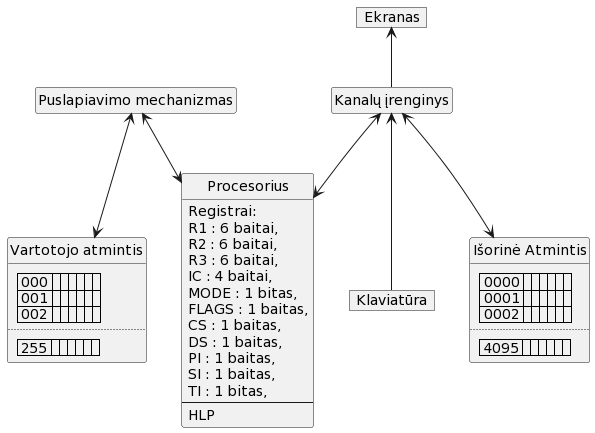
\includegraphics[scale=0.65]{img/reali_masina}
	\caption{Realios mašinos modelis}   % Antraštė įterpiama po paveikslėlio
	\label{img:reali_masina}
\end{figure}

\subsection{Procesorius}

Procesorius turi registrus:

\begin{itemize}
	\item IC - komandų skaitiklis - 2 baitai.
	\item R1, R2, R3 - bendrosios paskirties registrai iš 6 baitų (vienas žodis).
	\item CS - kodo segmento registras, 1 baitas.
	\item DS - duomenų segmento registras, 1 baitas.
	\item MODE - 1 bito registras, kuris nurodo procesoriaus darbo režimą (0 - vartotojas, 1 - supervizorius)
	\item FLAGS - 1 baito požymių registras, kurio reikšmė yra pakeičiama po aritmetinės ar palyginimo operacijos. Jis susideda iš šių bitų (numeruojami nuo jauniausio pradedant nuo skaičiaus 1): 
	\begin{itemize}
		\item (1-asis bitas) CF - pernešimo požymis (carry flag).
		\item (2-asis bitas) ZF - nulio požymis (zero flag).
		\item (3-asis bitas) SF - ženklo požymis (sign flag).
		\item (4-asis bitas) OF - perpildymo požymis (overflow flag).
		\item 5-asis, 6-asis, 7-asis ir 8-asis bitai nenaudojamas.
	\end{itemize}
	\item PTR - puslapiavimo registras - 2 baitai
	\item PI - 1 baito programinių pertraukimų registras.
	\item TI - 1 baito laikrodžio pertraukimas registras.
	\item SI - 1 baito sisteminių pertraukimų registras.
\end{itemize}

Be registrų procesorius dar turi Aukšto lygio kalbos procesorių - HLP. Jis atsakingas už komandų apdorojimą.

\subsection{Vartotojo atmintis}

Realios mašinos atminties dydis yra 256 blokai po 16 žodžių. Vieno žodžio ilgis yra 6 baitai.

\subsubsection{Puslapiavimas}

Norint virtualios mašinos blokų numerius paversti į realios mašinos blokų numerius yra taikomas puslapiavimo mechanizmas. Tam tikslui, kuriant virtualią mašiną, yra išskiriamas dar vienas blokas, kuriame saugama lentelė, atliekanti pervertimą.

Kai PTR reikšmė yra $a_0a_1$, kur $a_0, a_1$ yra šešioliktainiai skaičiai. Tada puslapių lentelės bloko adresas yra $16 * a_0 + a_1$  

Virtualaus adreso $x_0x_1$ ($x_0, \ x_1$ - šešioliktainiai skaičiai) realus adresas = $16 * [16*(16 * a_0 + a_1) + x_0] + x_1$.

\subsection{Supervizorinė atmintis}

Pirmi 16 realios mašinos blokų yra skiriami supervizorinei atminčiai.

\subsection{Pertraukimai}

Pertraukimą iškviečia vartotojas. Tada yra pakeičiama registro MODE reikšmė į 1 (supervizoriaus režimas) ir šiame režime yra vykdomas pertraukimas. 

Programiniai pertraukimai PI gali kilti, bandant įvykdyti kokį nors neleistiną veiksmą. Šie veiksmai yra:

\begin{itemize}
	\item PI = 1 - dalyba iš nulio.
	\item PI = 2 - netinkamas adresas.
	\item PI = 3 - neleistinas operacijos kodas
	\item PI = 4 - perpildymas
\end{itemize}

Sisteminiai pertraukimai SI:
\begin{itemize}
	\item SI = 1 - komanda HALT**
	\item SI = 2 - komanda OPENF*
	\item SI = 3 - komanda CLOSEF
	\item SI = 4 - komanda WRITEF
	\item SI = 5 - komanda READF*
	\item SI = 6 - komanda DELETF
	\item SI = 7 - komanda OUTSIM
	\item SI = 8 - komanda OUTNUM
	\item SI = 9 - komanda INPONE		
	\item SI = 10 - komanda INPBLK		
\end{itemize}

TI yra atsakingas už taimerio mechanizmą.

\subsubsection{Taimerio mechanizmas}
Realioje mašinoje yra taimeris. Jis skirtas tam, kad viena užduotis nebūtų vykdoma daugiau nei 10 laiko momentų. Tam tikslui po kiekvienos operacijos yra sumažina TI reikšmė. Taip pat skirtingos operacijos užtrunka kitokį laiko skaičių: išvedimo į kanalų įrenginį ar įvedimo į jį užima 5 laiko vienetus, o visos kitos - 1. Kai TI reikšmė pasiekia 0 yra sugeneruojamas taimerio pertraukimas.

\subsection{Kanalų įrenginys}

Realioje mašinoje yra įvedimo ir išvedimo įrenginys - atitinkamai klaviatūra ir  ekranas. Jie su procesorium apsikeičia duomenimis tik per kanalų įrenginį. Įvydžius komandą EXCHGE yra perkeliamas norimi baitai. Tam, kad būtų tiksliai specifikuota, tai, kas bus perkeliama yra naudojami šie kanalų įrenginio registrai:

\begin{itemize}
	\item SB - 2 baitų registras, kuriame saugomas bloko, iš kurio bus kopijuojama numeris. Registro reikšmė saugoma kaip šešioliktainis skaičius.
	\item SW - 2 baitų registras, nuo kurio baito takelyje bus kopijuojama. Pirmame baite kaip šešioliktainis skaičius nurodyta, nuo kurio žodžio kopijuojama. Antrame - saugoma nuo kurio baito tame žodyje bus kopijuojama (tarp 0 ir 5 imtinai).
	\item DB - 2 baitų registras, kuriame saugas bloko, į kurį bus kopijuojama numeris. Registro reikšmė saugoma kaip šešioliktainis skaičius.
	\item DW - 2 baitų registras, nuo kurio baito takelyje bus kopijuojama. Pirmame baite kaip šešioliktainis skaičius nurodyta, nuo kurio žodžio kopijuojama. Antrame - saugoma nuo kurio baito tame žodyje bus kopijuojama (tarp 0 ir 5 imtinai).
	\item BC - 2 baitų registras, kuriame nurodoma, kiek baitų bus kopijuojama. Registro Registro reikšmė saugoma kaip šešioliktainis skaičius.
	\item ST - 1 baito registras, kuriame nurodytas tipas objekto, kuris bus kopijuotas. ST esančio skaičiaus reikšmės:
	\begin{enumerate}
		\item Vartotojo atmintis
		\item Supervizorinė atmintis
		\item Išorinė atmintis
		\item Klaviatūra
	\end{enumerate}
	\item DT - 1 baito registras, kuriame nurodytas tipas objekto, į kurį bus kopijuojama. ST esančio skaičiaus reikšmės:
	\begin{enumerate}
		\item Vartotojo atmintis
		\item Supervizorinė atmintis
		\item Išorinė atmintis
		\item Ekranas
	\end{enumerate}
\end{itemize}

\subsection{Išorinė Atmintis}

Išorinė atmints yra realizuojama kietuoju disku. Jame yra 256 blokai po 16 žodžių.

Komunikacija su išorine atmintimi yra vykdoma per kanalų įrenginį.

\subsection{Klaviatūra}

Kiekvienas klaviatūros mygtuko paspaudimai yra operacinės sistemos saugomi iki programa juos pasiima. Pasiimimas vyksta per kanalų įrenginį.

\subsection{Ekranas}

Į ekraną yra išvedama tiek simbolių. Programa norėdama tai  atlikti turi nustatyti registrų reikšmes ir iškviesti atitinkamą sisteminį pertraukimą.

\section{Virtualios mašinos modelis}

Virtuali mašina - operacinės sistemos konstruktas, kurio pagalba kiekvienos programos veikimas yra izoliajamos nuo visų kitų, o darbui su bendrais įrenginiais pasitelkiama operacinė sistemą. Reali mašina paleidžia virtualią mašiną, o ši vykdo komandas. Šios mašinos modelis yra pateikiamas \ref{img:virtuali_masina} paveiksliuke.

\begin{figure}[H]
	\centering	
	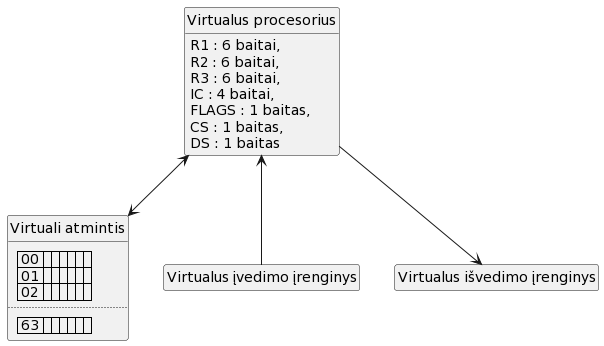
\includegraphics[scale=0.65]{img/virtuali_masina}
	\caption{Virtualios mašinos modelis}   % Antraštė įterpiama po paveikslėlio
	\label{img:virtuali_masina}
\end{figure}

\subsection{Registrai}

Virtuali mašina turi priėjimą tik prie šių realios mašinos registrų:

\begin{itemize}
	\item R1, R2, R3 (bendros paskirties registrai)
	\item CS (kodo segmento registras)
	\item DS (duomenų segmento registras)
	\item FLAGS (požymių registras)
	\item IC (programos skaitiklis)
\end{itemize}

\subsection{Atmintis}

Virtuali mašina turi priėjimą prie 16 blokų. Ji gauna jų virtualius numerius. Dėl to kiekviena virtuali mašina mato, kad jos blokai yra pirmi šešiolika - 0, 1, ..., 14, 15.

\subsection{Komandos}

Visos komandos yra aprašomos vienu žodžiu - 6 baitais. Visose komandose simbolis * reiškia, kad šis baitas nėra naudojamas.

\subsubsection{Aritmetinės}
\begin{itemize}
	\item ADDmxy - jei m = r, tai operacija sudeda skaičius esančius registruose Rx, Ry ir rezultatą patalpina į R1. Jei m=c, tai operaciją atlieka su registru Rx ir konstanta y. Antru atveju y yra šešioliktainis skaičius.
	\item SUBmxy - jei m = r, tai operacija atima iš skaičiaus esančio registre Rx, skaičių iš registro Ry ir rezultatą patalpina į R1. Jei m=c, tai operaciją atlieka su registru Rx ir konstanta y. Antru atveju y yra šešioliktainis skaičius.
	\item MULmxy - jei m = r, tai operacija sudaugina skaičius esančius registruose Rx, Ry ir rezultatą patalpina į R1. Jei m=c, tai operaciją atlieka su registru Rx ir konstanta y. Antru atveju y yra šešioliktainis skaičius.
	\item DIVmxy - jei m = r, tai operacija padalina skaičių esantį registre Rx, iš skaičiaus esančio registre Ry ir rezultatą patalpina į R1. Jei m=c, tai operaciją atlieka su registru Rx ir konstanta y. Antru atveju y yra šešioliktainis skaičius.
	\item CMPmxy - jei m = r, tai operacija palygina skaičius esančius registruose Rx ir Ry bei pagal Rx-Ry reikšmę nustato registro FLAGS reikšmę. Jei m=c, tai operaciją atlieka su registru Rx ir konstanta y. Antru atveju y yra šešioliktainis skaičius.
\end{itemize}

Po kiekvienos aritmetinės operacijos procesorius padina IC reikšmę. Taip pat po kiekvienos aritmetinės operacijos pagal rezultatą (o palyginimo atveju - lyginamųjų skaičių skirtumą) yra nustatomos registro FLAGS reikšmės.

\begin{itemize}
	\item CF: Nustatomas 1, jei yra pernešimas ar skolinimasis iš vyriausiojo bito, kitu atveju - 0.
	\item ZF: Jei rezultatas yra 0, tai nustatomas ZF = 1, kitu atveju ZF = 0.
	\item SF: Jei vyriausias bitas yra 1, tai nustatoma SF = 1, kitu atveju SF = 0.
	\item OF: Nustatomas 1, jei rezultatas per didelis teigiamas ar permažas neigiamas, kad tilpų į rezultatą nenaudojant ženklo bitu, kitu atveju - 0.
\end{itemize}

\subsubsection{Duomenų judėjimo}
\begin{itemize}
	\item MVmrxy - Perkelia duomenis. m reikšmė nurodo perkelimo režimą. x ir y specifikuoja vietas, kur juda duomenys. Po šios komandos yra padidinama IC reikšmė. Čia x ir y yra šešioliktainiai skaičiai.
	\begin{enumerate}
		\item m = r. Šiuo atveju perkėlimas yra iš registro į registrą. x nurodo pirmo registro (šaltinio) numerį, y - tikslo. Šiuo atveju r reikšmė nenaudojama
		\item m = o. Šiuo atveju perkėlimas yra iš registro į atmintį. Atminties vieta yra gaunama pagal formulę $10_{16} \cdot x + y$, o registro numeris - pagal r reikšmę
		\item m = i. Šiuo atveju perkėlimas yra iš atminties į registrą. Atminties vieta yra gaunama pagal formulę $10_{16} \cdot x + y$, o registro numeris - pagal r reikšmę
		\item m = c. Šiuo atveju į registrą yra perkeliama konstanta. Registro numerį nurodo r, o konstanta yra $10_{16} \cdot x + y$, kur x, y - šešioliktainiai skaičiai. Konstanta pakeičia registro žemiausią baitą, o likę išlieka nepakitę.
	\end{enumerate}
\end{itemize}


Registrai yra numeruojami taip:
\begin{enumerate}
	\item R1
	\item R2
	\item R3
	\item CS
	\item DS
\end{enumerate}

\subsubsection{Valdymo}
Norint tinkamai naudotis perėjimais, prieš juos reikia panaudoti CMP operaciją. Komandose naudojami x, y, z yra šešioliktainiai skaičiai
\begin{itemize}
	\item JMPxy* - besąlyginis perėjimas. Pakeičia $ \text{IC} := 10_{16} * \text{x} + \text{y}$
	
	\item JExy** - pereiti, jeigu lygu. Jei ZF=1, tai $ \text{IC} := 10_{16} * \text{x} + \text{y}$, kitu atveju IC := IC + 1.
	\item JNExy* - pereiti, jei nelygu. Jei ZF=0, tai $ \text{IC} := 10_{16} * \text{x} + \text{y}$, kitu atveju IC := IC + 1.
	
	\item JLxy** - pereiti, jeigu mažiau (su ženklu). Jei SF$\neq$OF, tai $ \text{IC} := 10_{16} * \text{x} + \text{y}$, kitu atveju IC := IC + 1.
	\item JLExy* - pereiti, jeigu mažiau arba lygu (su ženklu). Jei ZF=1 arba SF$\neq$OF, tai $ \text{IC} := 10_{16} * \text{x} + \text{y}$, kitu atveju IC := IC + 1.
	\item JGxy** - pereiti, jeigu daugiau (su ženklu). Jei ZF=0 arba SF=OF, tai $ \text{IC} := 10_{16} * \text{x} + \text{y}$, kitu atveju IC := IC + 1.
	\item JGExy* - pereiti jeigu daugiau arba lygu (su ženklu). Jei SF=OF, tai $ \text{IC} := 10_{16} * \text{x} + \text{y}$, kitu atveju IC := IC + 1.
	
	\item JBxy** - pereiti, jei žemiau (be ženklo). Jei CF=1, tai $ \text{IC} := 10_{16} * \text{x} + \text{y}$, kitu atveju IC := IC + 1.
	\item JBExy* - pereiti, jei žemiau ar lygu (be ženklo). Jei CF=1 arba ZF=1, tai $ \text{IC} := 10_{16} * \text{x} + \text{y}$, kitu atveju IC := IC + 1.
	\item JAxy** - pereiti, jei aukščiau (be ženklo). Jei CF=0 ir ZF = 0, tai $ \text{IC} := 10_{16} * \text{x} + \text{y}$, kitu atveju IC := IC + 1.
	\item JAExy* - pereiti, jei aukščiau arba lygu (be ženklo). Jei CF = 0, tai $ \text{IC} := 10_{16} * \text{x} + \text{y}$, kitu atveju IC := IC + 1.
\end{itemize}

Po valdymo komandų registro FLAGS reikšmė nėra keičiama.

\subsubsection{Darbas su failais}
Darbo su failais metu yra naudojamos simbolių eilutės. Tai baitų seka, kurios pabaigoje yra nulinis baitas.

Visos šios operacijos iškviečia sisteminius pertraukimus. Procesorius informaciją apie pertraukimo tipą gauna iš SI reikšmės.
\begin{itemize}
	\item OPENF* - atidaro failą, kurio pavadinimas yra simbolių eilutė, kurios pradžios adresas yra R1 reikšmė. Operacijos pabaigoje į R2 yra įrašomas failo numeris. Jeigu failas yra nerandamas - sukuria naują failą tokiu pavadinimu.
	\item CLOSEF - uždaro failą, kurio numeris yra įrašytas  R2. Jeigu norimas failas nėra rastas, ar jau buvo uždarytas yra nustatoma R1 = 0, kitu atveju R1 bus uždaryto failo numeris.
	\item WRITEF - rašo simbolius į failą, kurio numeris nurodytas R2. Rašoma nuo adreso, kuris nurodytas R1 iki tol, kol parašo R3 baitų arba sutinkamas nulinis baitas.
	\item READF* - skaito simbolius iš failo, kurio numeris yra nurodytas R2. Rašymas į atmintį pradedamas nuo vietos, kurią nurodo R1 reikšmė. Perskaitomi baitai iki failo galo, bet nedaugiau negu buvo nurodyta reikšmėje R3. Jeigu buvo perskaityta mažiau, negu buvo nurodyta R3 reikšmėje, tai ji atitinkamai pakeičiama.
	\item DELETF - sunaikiną failą, kurio numeris nurodomas R2 reikmšmėje. Jeigu norimas failas nebeegzistuoja arba nepavyksta jo sunaikinti - operacijos pabaigoje įrašo į R2 reikšmę 0, kitu atveju nekeičia R2 reikšmės. Sunaikinus failą jo nereikia uždarinėti.
\end{itemize}

Po kiekvienos iš šių komandų procesorius padidina registro IC reikšmę.

Naują eilutę darbe su failais bei įvedime ir išvedime žymi du simboliai \\n.

Jeigu WRITEF nepavyko parašyti visų simbolių, tai yra nustatomas CF = 1, o priešingu atveju CF reikšmė yra išvaloma. Kitos valdymo komandos nekeičia registro FLAGS reikšmės.

\subsubsection{Įvedimas ir išvedimas}
Įvedimo ir išvedimo komandos, kaip ir darbo su failais, iškviečia sisteminį pertraukimą. 
\begin{itemize}
	\item OUTSIM - išveda baitus nuo R1 nurodyto adreso iki kol sutinka nulinį baitą arba parašo tiek simbolių, kokia reikšmė dabar yra registre R3.
	\item OUTNUM - išveda baitą, kuris nurodytas R1 kaip skaičių.
	\item INPONE - perskaito simbolį iš įvedimo srauto bei reikšmę patalpina į R1. Iki kol simbolis yra įvedamas, programa užsiblokuoja. Jeigu nuskaityti nepavyko, tai gauname reikšmė R1=0.
	\item INPBLK - perskaito 16 simbolių (vieną takelį) iš įvedimo srauto ir patalpina į atmintį, nuo adreso, nurodyto registre R1. Kol takelis nėra gaunamas, programa užsiblokuoja.
\end{itemize}

\subsubsection{Programos pabaigos}
\begin{itemize}
	\item HALT** - iškviečia sisteminį pertraukimą, kuris baigia programos darbą.
\end{itemize}

\subsection{Programos struktūra}

Maksimalus programos dydis yra 256 žodžiai, t.y. 16 blokų. Failo pavadinimas gali būti tik vieno žodžio.

Programos pradžią žymi žodis \$PROG\$. Po jo yra pavadinimas, o žymė ------ (šeši '-' ženklai) - pavadinimo pabaigą. Ši dalis užima pirmąjį takelį. Taip pat pabaigos žymė turi būti viename žodyje.

Prieš kiekvieną naują programos ar duomenų bloką turi būti žymė. Žymės yra vienos iš dviejų tipų: pozicinės ir vardinės.

Pozicinės yra aprašomas formatu \$\$x\$\$\$, kur x yra šešioliktainis skaičius, nurodantis takelio numerį (numeruojama nuo 0), į kurį bus rašomi duomenys.

Vardinės yra dvi žymės: .CODES ir .DATAS, kurios atitinkamai reiškia kodo segmentą ir duomenų segmentą. Jos taip pat atinkama pozicines žymes \$\$1\$\$\$ ir \$\$8\$\$\$. Programoje šių žymių gali ir nebūti.

Kodo segmentas ypatingas tuo, kad visos reikšmės patenkančios į jį yra perkeliamos į programą.

Programos darbo pradžioje yra nustatomos tokios reikšmės: IC = $10_{16}$, CS = $10_{16}$, DS = $80_{16}$.

Programos pabaiga žymi žodis \$FINS\$. 

\subsection{Failo struktūra}

Failo maksimalus dydis yra neribojamas, tačiau failo pavadinimas yra vienas žodis.

Failo pradžią žymi žodis \$FILE\$. Po jo yra failo pavadinimas, o žymė ------ (šeši '-' ženklai) žymi pavadinimo pabaigą. 

Po jų seka failas. Jis yra baigiamas žodžiu \$FINS\$

\subsection{Išorinio disko pavyzdys}

Išorinėje atmintyje duomenys saugomi failais ir programomis. Laikoma, kad visa atmintis, kuri netenkina aprašytos struktūros yra ignoruojama.

Žemiau nurodomas galimas kietojo disko pavyzdys su trimis programomis:

\begin{enumerate}
	\item "ciklas" - programa vykdanti amžinąjį ciklą.
	\item "sudeti" - iš vartotojo įvesties gauna du skaičius ir išveda jų sumą.
	\item "jungti" - iš vartotojo įvesties gauna dviejų failų pavadinimus, skaito juose esantį tekstą ir sujungtą failą "sujungtas" (pradžioje pirmo, tada antro). Jei trečiasis failas pradžioje buvo netuščias, tai jį ištrina.
\end{enumerate}

\begin{verbatim}
	
$PROG$
ciklas
------
.CODES
JMP10*
.DATAS
$FINS$
$PROG$
sudeti
------
.CODES
MVrr51
MVc318
OUTPUT
INPONE
MVrr12
MVc190
MVc318
OUTPUT
INPONE
ADD012
MVrr12
MVc1F0
MVc30B
MVrr21
OUTNUM
.DATAS
iveski
te pir
ma ska
iciu\n
$$9$$$
iveski
te ant
ra ska
iciu\n
$$A$$$
gauta 
suma:  
$FINS$
$PROG$
jungti
------
.CODES
MVc1A0
MVo2C0
OPENF*
DELETF
MVrr41
MVc31B
OUTPUT
MVc1A0
MVc310
INPBLK
OPENF*
MVo2C1
MVi2C1
READF*
MVi2C0
WRITEF
CMPc30
JE15**
MVi2C1
CLOSEF
MVrr41
MVc31B
OUTPUT
MVc1A0
MVc310
INPBLK
OPENF*
MVo2C1
MVi2C1
READF*
MVi2C0
WRITEF
CMPc30
JE20**
MVi2C1
CLOSEF
MVi2C0
CLOSEF
.DATAS
Iveski
te fai
lo pav
adinim
a\n
$$A$$$
sujung
tas   
$FILE$
pirmas
------
pirmoj
o fail
o eilu
tes, k
urios 
reikal
ingos 
jungim
ui.   
$FINS$
$FILE$
antras
------
antroj
o fail
o eilu
tes, k
urios 
reikal
ingos 
jungim
ui.   
$FINS$
\end{verbatim}

\subsection{Virtuali mašina operacinės sistemos kontekste}

Operacinė sistema paleidžia virtualią mašiną kiekvienai programai. Jei operacinė sistema yra multiprograminė, tai joje vienu metu veikia tik viena programa, bet vykdomoji programa nuolatos keičiasi.

Virtualias mašinas kuria operacinė sistemą. Jos yra sukuriamos, kai vartotojas įveda programą LOAD prg, kur prg yra programos pavadinimas kietąjame diske. Tada programa yra perkeliama į supervizorinę atmintį, joje yra patikrinama ar programoje nėra neegzistuojančių komandų. Jei yra - įkėlimas nutraukiamas, jei nėra - programa perkeliama į vartotojo atmintį.

Pažingsniui kūrimo scenarijus būtų toks:

\begin{enumerate}
	\item Pradedama kurti virtuali mašina.
	\item Ji reikalauja 16 takelių.
	\item Išskiriamas papildomas takelis puslapių lentelei, kuris užpildomas adresais.
	\item Nustatoma registro PTR reikšmė su puslapių lentelės adresu.
	\item Virtuali mašina baigiama kurti ir gauna procesorių.
\end{enumerate}

\printbibliography[heading=bibintoc] % Literatūros šaltiniai aprašomi
\appendix  % Priedai

\end{document}
